%%%%%%%%%%%%%%%%%%%%%%%%%%%%%%%%%%%%%%%%%
% APA Assignment Article
% LaTeX Template
% Version 2.0 (February 7, 2023)
%
% This template originates from:
% https://www.LaTeXTemplates.com
%
% Author:
% Vel (vel@latextemplates.com)
%
% License:
% CC BY-NC-SA 4.0 (https://creativecommons.org/licenses/by-nc-sa/4.0/)
%
% NOTE: The bibliography needs to be compiled using the biber engine.
%
%%%%%%%%%%%%%%%%%%%%%%%%%%%%%%%%%%%%%%%%%

%----------------------------------------------------------------------------------------
%	PACKAGES AND OTHER DOCUMENT CONFIGURATIONS
%----------------------------------------------------------------------------------------

\documentclass[
	letterpaper, % Paper size, use either a4paper or letterpaper
	10pt, % Default font size, can also use 11pt or 12pt, although this is not recommended
	unnumberedsections, % Comment to enable section numbering
	twoside, % Two side traditional mode where headers and footers change between odd and even pages, comment this option to make them fixed
]{APAAssignment}

\addbibresource{bibliography.bib} % BibLaTeX bibliography file

\runninghead{MICS CYBER 252, Fall-2024 Hands On Lab Unit 7} % A shortened article title to appear in the running head, leave this command empty for no running head

\footertext{\textit{Hands On Lab 7} (MICS CYBER 252, Fall -2024)} % Text to appear in the footer, leave this command empty for no footer text

\setcounter{page}{1} % The page number of the first page, set this to a higher number if the article is to be part of an issue or larger work

%----------------------------------------------------------------------------------------
%	TITLE SECTION
%----------------------------------------------------------------------------------------

\usepackage[title,toc,titletoc]{appendix}
\usepackage{titlesec}
\usepackage{lscape}
\usepackage{fontawesome}

\title{Hands On Lab: Unit 7 \\ MICS-252, Fall 2024 \\ Threat Detection} % Article title, use manual lines breaks (\\) to beautify the layout

% Authors are listed in a comma-separated list with superscript numbers indicating affiliations
% \thanks{} is used for any text that should be placed in a footnote on the first page, such as the corresponding author's email, journal acceptance dates, a copyright/license notice, keywords, etc
% Affiliations are output in the \date{} command
\date{UC Berkleley School of Information \\
MICS Course 252 Fall 2024 (Kristy Westphal)
}


\author{
	Prepared by: Karl-Johan Westhoff \\
	email: \href{mailto:kjwesthoff@berkeley.edu}{kjwesthoff@berkeley.edu}
}


% % Full-width abstract
% \renewcommand{\maketitlehookd}{%
% 	\begin{abstract}
% 		\noindent Lorem ipsum dolor sit amet,rta porttitor.
% 	\end{abstract}
% }

%----------------------------------------------------------------------------------------

\setcounter{tocdepth}{5}
\setcounter{secnumdepth}{5}
\usepackage[title]{appendix}

\begin{document}
\onecolumn
\maketitle % Output the title section

%----------------------------------------------------------------------------------------
%	ARTICLE CONTENTS
%----------------------------------------------------------------------------------------


\section{Introduction}
In the previous Assignment unit 6 \cite{Assingnment6} the 'home network' threat model using 'STRIDE' identified the following weaknesses:

\begin{spacing}{1}
	\begin{itemize}
		\item Exploitable assets, allowing access to the network and pivot points for further exploitation
		\item WIFI passwords may have been leaked granting direct access to the network
		\item Logging is scarce, inconsistent and incoherent (Windows pc's may log a-lot, IOT devices may not log at all, logging at the NAT is limited)
	\end{itemize}
\end{spacing}

\section{What Are We Protecting from What?}
We are protecting on our home network:
\begin{spacing}{1}
	\begin{itemize}
		\item Our login credentials (Bank, Online services etc.)
		\item Personal data (Documents, images etc.)
		\item Privacy (online activity)
		\item Use of your bandwidth (cost and speed)
	\end{itemize}
\end{spacing}

The threats are:

\begin{spacing}{1}
	\begin{itemize}
		\item Phishing attacks to steal credentials
		\item Malware ('old fashioned' viruses, key loggers etc.)
		\item Assets being utilized as zombies in a botnet (botnets, crypto mining, etc.)
		\item Uncontrolled hosts on network
	\end{itemize}
\end{spacing}


\section{Treat Control Use Cases}

Applying the:
\begin{spacing}{1}
	\begin{enumerate}
		\item Indicator
		\item Data Source
		\item Action
	\end{enumerate}
\end{spacing}
Methodology to each identified threat, gives some possible 'Use Cases'\footnote{I am a bit puzzled by the term 'Use Case' as it sounds like a sales argument for a SIEM, I think 'Threat Control' is a better term and can be applied holistically} for detection rules.

\subsection{Phishing}
Use case Outcome: Detect and block inbound phishing
\begin{spacing}{1}
	\begin{itemize}
		\item Indicators:
		      \begin{itemize}
			      \item Suspicious sender
			      \item Suspicious domain (could be subtle changes to a URL)
			      \item Unusual requests e.g asking for SSN, bank account number etc.
		      \end{itemize}
		\item Data Source:
		      \begin{itemize}
			      \item Email vendor/service provider phishing detection and filtering (they maintain the signatures and notifies)
			      \item Endpoint protection (e.g. Windows defender\cite{WindowsDefenderCommercial}), with an updated list of signatures
		      \end{itemize}
		\item Action:
		      \begin{itemize}
			      \item Hold
			      \item Block/Drop (in case of known phishing sender/domain)
			      \item Alert
		      \end{itemize}
	\end{itemize}
\end{spacing}

\subsection{Malware}
Use case Outcome: Detect malware and notify user at host level
\begin{spacing}{1}
	\begin{itemize}
		\item Indicators:
		      \begin{itemize}
			      \item Endpoint protection (virus detection)
			      \item Unusual behavior (slowing down)
		      \end{itemize}
		\item Data Source:
		      \begin{itemize}
			      \item Endpoint protection logs and notifications (EDR if equipped)
			      \item Network detection (NDR if equipped)
		      \end{itemize}
		\item Action:
		      \begin{itemize}
			      \item Block
			      \item Alert
		      \end{itemize}
	\end{itemize}
\end{spacing}

\subsection{DDOS zombie}
Use Case Outcome: Notify network administrator (you) that botnet traffic is emerging from your public IP

\begin{spacing}{1}
	\begin{itemize}
		\item Indicators:
		      \begin{itemize}
			      \item Unusual behavior (slowness, the user is the detection system here)
			      \item Get notified from outside\footnote{DDOS is difficult to detect, if you are part of a botnet you will likely just get the traffic going to the attacked endpoint blocked and never know about it, a mitigation may be a notification service.}
		      \end{itemize}
		\item Data Source:
		      \begin{itemize}
			      \item Endpoint protection (EDR if equipped)
			      \item Network detection (NDR if equipped)
		      \end{itemize}
		\item Action:
		      \begin{itemize}
			      \item Alert
			      \item Block
		      \end{itemize}
	\end{itemize}
\end{spacing}

\subsection{Unwanted hosts on network}
Use Case outcome: Block unauthorized hosts on network
\begin{spacing}{1}
	\begin{itemize}
		\item Indicators:
		      \begin{itemize}
			      \item Unexpected host logging onto network
		      \end{itemize}
		\item Data Source:
		      \begin{itemize}
			      \item NAT/DHCP server log and firewall policy
		      \end{itemize}
		\item Action:
		      \begin{itemize}
			      \item Block if not on approved MAC list
		      \end{itemize}
	\end{itemize}
\end{spacing}



\section{Conclusion}
Home networks are limited regarding infrastructure to detect and protect network activity and relies more on passive measures, such as subnetting and protection of individual endpoints. Home networks requirements are both simple (providing basic HTTP/S access) and complicated (providing services and protocols making things like printers simple to use). Furthermore, IOT complicates the security management, the chip sets used are cheap but still capable of doing actual computing, making them targets for use in zombie botnets.
Apart from 'static' remedies such as subnetting, implementing real monitoring of the network requires some knowledge which the normal consumer does not have. \\
Discovering and alerting of botnets is delegated to large entities which have an overview of a network and resources to kill DDOS at a many points around the network \cite{CloudFlareDDOS}. \\
Some automated firewall and network detection and response 'boxes'\cite{FireWallaCommerical} are available to home network users with monitoring of bandwidth usage, blocking phishing, advertisement and network events. Anyway these are not 'deploy and forget' some interaction is required to interpret alerts. \\
Monitoring on a home networks could be allocated to the extremes of the data flow, and regard the network itself as an insecure place. Monitoring of bank transactions often happen on the bank's infrastructure, and monitoring of privacy is allocated to the endpoints on the network (things with web browsers) \\
Even tough the 'STRIDE' model is primarily minded for software systems, I think it actually works well for home networks with a bit of adaptation, I guess something like a home network actually resembles a system with well defined boundaries like a piece of software. The STRIDE analysis provided clear weaknesses which could then be used to define vulnerabilities for which detection mechanisms can be defined using the Indicator -> Data Source -> Action template.


















%\begin{figure}[!htp] % Single column :figure	
%	\centering
% 	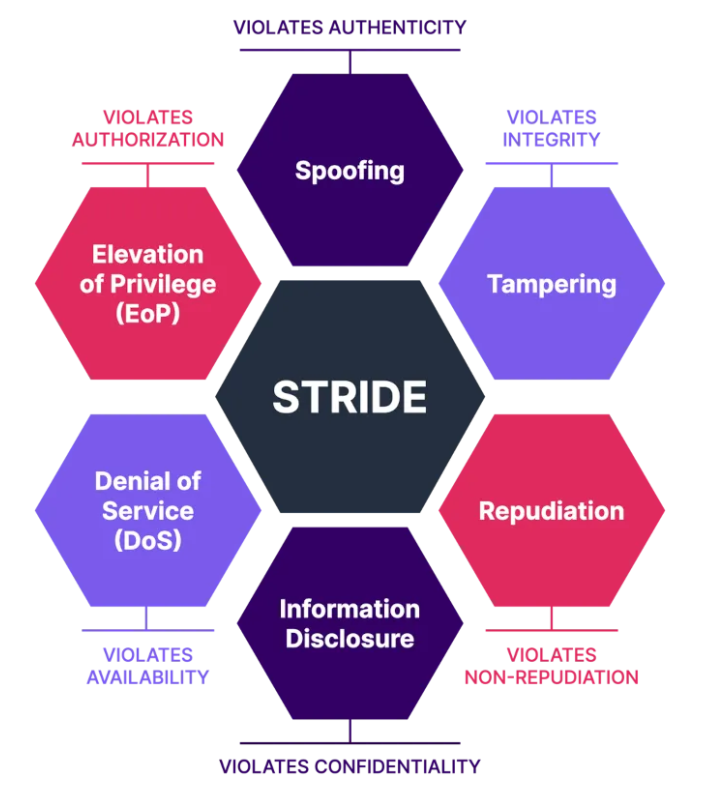
\includegraphics[width=0.5\linewidth]{STRIDE.png}
% 	\caption{The STRIDE model summarized, illustration from \cite{STRIDE_For_pay_Medium}}
% 	\label{fig:STRIDE}
% \end{figure}
%

%----------------------------------------------------------------------------------------
%	 REFERENCES
%----------------------------------------------------------------------------------------

\printbibliography % Output the bibliography

%----------------------------------------------------------------------------------------



%----------------------------------------------------------------------------------------
%	 Appendices
%----------------------------------------------------------------------------------------

% \appendix


% \clearpage
% \chapter{Appendices}
% \begin{appendices}

% \end{appendices}
\end{document}
